% Options for packages loaded elsewhere
\PassOptionsToPackage{unicode}{hyperref}
\PassOptionsToPackage{hyphens}{url}
%
\documentclass[
  english,
  a4paper,floatsintext]{apa7}
\usepackage{amsmath,amssymb}
\usepackage{lmodern}
\usepackage{iftex}
\ifPDFTeX
  \usepackage[T1]{fontenc}
  \usepackage[utf8]{inputenc}
  \usepackage{textcomp} % provide euro and other symbols
\else % if luatex or xetex
  \usepackage{unicode-math}
  \defaultfontfeatures{Scale=MatchLowercase}
  \defaultfontfeatures[\rmfamily]{Ligatures=TeX,Scale=1}
  \setmainfont[]{Times New Roman}
\fi
% Use upquote if available, for straight quotes in verbatim environments
\IfFileExists{upquote.sty}{\usepackage{upquote}}{}
\IfFileExists{microtype.sty}{% use microtype if available
  \usepackage[]{microtype}
  \UseMicrotypeSet[protrusion]{basicmath} % disable protrusion for tt fonts
}{}
\makeatletter
\@ifundefined{KOMAClassName}{% if non-KOMA class
  \IfFileExists{parskip.sty}{%
    \usepackage{parskip}
  }{% else
    \setlength{\parindent}{0pt}
    \setlength{\parskip}{6pt plus 2pt minus 1pt}}
}{% if KOMA class
  \KOMAoptions{parskip=half}}
\makeatother
\usepackage{xcolor}
\IfFileExists{xurl.sty}{\usepackage{xurl}}{} % add URL line breaks if available
\IfFileExists{bookmark.sty}{\usepackage{bookmark}}{\usepackage{hyperref}}
\hypersetup{
  pdftitle={DoPL},
  pdfauthor={Ithurburn, Andrew1, Pedersen, Julie1, \& Moore, Adam1},
  pdflang={en-EN},
  pdfkeywords={keywords},
  hidelinks,
  pdfcreator={LaTeX via pandoc}}
\urlstyle{same} % disable monospaced font for URLs
\usepackage{graphicx}
\makeatletter
\def\maxwidth{\ifdim\Gin@nat@width>\linewidth\linewidth\else\Gin@nat@width\fi}
\def\maxheight{\ifdim\Gin@nat@height>\textheight\textheight\else\Gin@nat@height\fi}
\makeatother
% Scale images if necessary, so that they will not overflow the page
% margins by default, and it is still possible to overwrite the defaults
% using explicit options in \includegraphics[width, height, ...]{}
\setkeys{Gin}{width=\maxwidth,height=\maxheight,keepaspectratio}
% Set default figure placement to htbp
\makeatletter
\def\fps@figure{htbp}
\makeatother
\setlength{\emergencystretch}{3em} % prevent overfull lines
\providecommand{\tightlist}{%
  \setlength{\itemsep}{0pt}\setlength{\parskip}{0pt}}
\setcounter{secnumdepth}{-\maxdimen} % remove section numbering
% Make \paragraph and \subparagraph free-standing
\ifx\paragraph\undefined\else
  \let\oldparagraph\paragraph
  \renewcommand{\paragraph}[1]{\oldparagraph{#1}\mbox{}}
\fi
\ifx\subparagraph\undefined\else
  \let\oldsubparagraph\subparagraph
  \renewcommand{\subparagraph}[1]{\oldsubparagraph{#1}\mbox{}}
\fi
\newlength{\cslhangindent}
\setlength{\cslhangindent}{1.5em}
\newlength{\csllabelwidth}
\setlength{\csllabelwidth}{3em}
\newlength{\cslentryspacingunit} % times entry-spacing
\setlength{\cslentryspacingunit}{\parskip}
\newenvironment{CSLReferences}[2] % #1 hanging-ident, #2 entry spacing
 {% don't indent paragraphs
  \setlength{\parindent}{0pt}
  % turn on hanging indent if param 1 is 1
  \ifodd #1
  \let\oldpar\par
  \def\par{\hangindent=\cslhangindent\oldpar}
  \fi
  % set entry spacing
  \setlength{\parskip}{#2\cslentryspacingunit}
 }%
 {}
\usepackage{calc}
\newcommand{\CSLBlock}[1]{#1\hfill\break}
\newcommand{\CSLLeftMargin}[1]{\parbox[t]{\csllabelwidth}{#1}}
\newcommand{\CSLRightInline}[1]{\parbox[t]{\linewidth - \csllabelwidth}{#1}\break}
\newcommand{\CSLIndent}[1]{\hspace{\cslhangindent}#1}
% Manuscript styling
\usepackage{upgreek}
\captionsetup{font=singlespacing,justification=justified}

% Table formatting
\usepackage{longtable}
\usepackage{lscape}
% \usepackage[counterclockwise]{rotating}   % Landscape page setup for large tables
\usepackage{multirow}		% Table styling
\usepackage{tabularx}		% Control Column width
\usepackage[flushleft]{threeparttable}	% Allows for three part tables with a specified notes section
\usepackage{threeparttablex}            % Lets threeparttable work with longtable

% Create new environments so endfloat can handle them
% \newenvironment{ltable}
%   {\begin{landscape}\begin{center}\begin{threeparttable}}
%   {\end{threeparttable}\end{center}\end{landscape}}
\newenvironment{lltable}{\begin{landscape}\begin{center}\begin{ThreePartTable}}{\end{ThreePartTable}\end{center}\end{landscape}}

% Enables adjusting longtable caption width to table width
% Solution found at http://golatex.de/longtable-mit-caption-so-breit-wie-die-tabelle-t15767.html
\makeatletter
\newcommand\LastLTentrywidth{1em}
\newlength\longtablewidth
\setlength{\longtablewidth}{1in}
\newcommand{\getlongtablewidth}{\begingroup \ifcsname LT@\roman{LT@tables}\endcsname \global\longtablewidth=0pt \renewcommand{\LT@entry}[2]{\global\advance\longtablewidth by ##2\relax\gdef\LastLTentrywidth{##2}}\@nameuse{LT@\roman{LT@tables}} \fi \endgroup}

% \setlength{\parindent}{0.5in}
% \setlength{\parskip}{0pt plus 0pt minus 0pt}

% Overwrite redefinition of paragraph and subparagraph by the default LaTeX template
% See https://github.com/crsh/papaja/issues/292
\makeatletter
\renewcommand{\paragraph}{\@startsection{paragraph}{4}{\parindent}%
  {0\baselineskip \@plus 0.2ex \@minus 0.2ex}%
  {-1em}%
  {\normalfont\normalsize\bfseries\itshape\typesectitle}}

\renewcommand{\subparagraph}[1]{\@startsection{subparagraph}{5}{1em}%
  {0\baselineskip \@plus 0.2ex \@minus 0.2ex}%
  {-\z@\relax}%
  {\normalfont\normalsize\itshape\hspace{\parindent}{#1}\textit{\addperi}}{\relax}}
\makeatother

% \usepackage{etoolbox}
\makeatletter
\patchcmd{\HyOrg@maketitle}
  {\section{\normalfont\normalsize\abstractname}}
  {\section*{\normalfont\normalsize\abstractname}}
  {}{\typeout{Failed to patch abstract.}}
\patchcmd{\HyOrg@maketitle}
  {\section{\protect\normalfont{\@title}}}
  {\section*{\protect\normalfont{\@title}}}
  {}{\typeout{Failed to patch title.}}
\makeatother
\shorttitle{Title}
\keywords{keywords\newline\indent Word count: 1593}
\usepackage{csquotes}
\raggedbottom
\setlength{\parindent}{2em}
\setlength{\parskip}{0em}
\usepackage[switch]{lineno}
\linenumbers
\ifXeTeX
  % Load polyglossia as late as possible: uses bidi with RTL langages (e.g. Hebrew, Arabic)
  \usepackage{polyglossia}
  \setmainlanguage[]{english}
\else
  \usepackage[main=english]{babel}
% get rid of language-specific shorthands (see #6817):
\let\LanguageShortHands\languageshorthands
\def\languageshorthands#1{}
\fi
\ifLuaTeX
  \usepackage{selnolig}  % disable illegal ligatures
\fi

\title{DoPL}
\author{Ithurburn, Andrew\textsuperscript{1}, Pedersen, Julie\textsuperscript{1}, \& Moore, Adam\textsuperscript{1}}
\date{}


\authornote{

Add complete departmental affiliations for each author here. Each new line herein must be indented, like this line.

Enter author note here.

The authors made the following contributions. Ithurburn, Andrew: Conceptualization, Writing - Original Draft Preparation, Writing - Review \& Editing; Moore, Adam: Writing - Review \& Editing.

Correspondence concerning this article should be addressed to Ithurburn, Andrew, 7 George Square, Edinburgh, EH8 9JZ. E-mail: \href{mailto:a.ithurburn@sms.ed.ac.uk}{\nolinkurl{a.ithurburn@sms.ed.ac.uk}}

}

\affiliation{\vspace{0.5cm}\textsuperscript{1} The University of Edinburgh}

\abstract{
One or two sentences providing a \textbf{basic introduction} to the field, comprehensible to a scientist in any discipline.

Two to three sentences of \textbf{more detailed background}, comprehensible to scientists in related disciplines.

One sentence clearly stating the \textbf{general problem} being addressed by this particular study.

One sentence summarizing the main result (with the words ``\textbf{here we show}'' or their equivalent).

Two or three sentences explaining what the \textbf{main result} reveals in direct comparison to what was thought to be the case previously, or how the main result adds to previous knowledge.

One or two sentences to put the results into a more \textbf{general context}.

Two or three sentences to provide a \textbf{broader perspective}, readily comprehensible to a scientist in any discipline.
}



\begin{document}
\maketitle

\hypertarget{introduction}{%
\section{Introduction}\label{introduction}}

Throughout political history tyrants and despots have influenced great power over large swaths of land and communities. One common thread amongst these individuals are how they wield their great power, often through dominant tactics such as threats and political subversions. Recent history has shown with individuals like Donald Trump, Jair Bolsonaro, and Rodrigo Duterte who display authoritarian traits often wield their power through fear and threats of violence.

\hypertarget{dominance-prestige-and-leadership-orientation}{%
\subsection{Dominance, Prestige, and Leadership orientation}\label{dominance-prestige-and-leadership-orientation}}

Research in power desire motives have focused on three sub-domains: dominance, leadership, and prestige (Suessenbach et al., 2019). Each of these three different power motives are explanations as to different ways or methods that individuals in power sought power or were bestowed upon them.

\hypertarget{dominance}{%
\subsubsection{\texorpdfstring{\emph{Dominance}}{Dominance}}\label{dominance}}

The dominance motive is one of the more researched methods and well depicted power motives. Individuals with a dominance orientation display the more primal of human behavior. These individuals will seek power through direct methods such as asserting dominance, control over resources, or physically assaulting someone (Johnson et al., 2012; Winter, 1993). Early research in dominance motives has shown that acts of dominance ranging from asserting physical dominance over another to physical displays of violence has been shown in many mammalian species, including humans (citation needed).
Individuals high in dominance are often high in machiavellianism, narcissism, and often are prone to risky behavior (discussion further in the next section). Continued research has hinted at a possible tendency for males to display these dominant seeking traits more than females (citation needed). When high dominance individuals assert themselves they are doing so to increase their own individual sense of power (citation needed). Asserting ones own sense of dominance over another can be a dangerous task. In the animal kingdom it can often leader to injury. While, in humans asserting dominance can take a multitude of actions such as leering behaviors, physical distance, or other non-verbal methods to display dominance (citation needed). Power from a dominance perspective is often never bestowed upon someone. Often, high dominance individuals will take control and hold onto it.

\hypertarget{prestige}{%
\subsubsection{\texorpdfstring{\emph{Prestige}}{Prestige}}\label{prestige}}

Contrary to the dominance motivation of using intimidation and aggression to gain more power, a prestige motivation or prestige in general is bestowed upon an individual from others in the community (citation needed). Differently from the dominance motivation, a prestige motivation is generally unique to the human species (citation needed). Due in part to ancestral human groups being smaller hunter-gatherer societies, individuals that displayed and used important behaviors beneficial to the larger group were often valued and admired by the group. Therein, the social group bestows the authority onto the individual. Generally, this type of behavior can be passively achieved by the prestigious individual. However, this does not remove the intent of the actor in that they too can see prestige from the group, but method of achieving that social status greatly differs from that of dominance seeking individuals.
Apart from dominance motivated individuals that continually have to fight for their right to have power over others, individuals that seek or were given power through a prestige motivation are not generally challenged in the same sense as dominant individuals. Displaying behaviors that the community would see as beneficial would indere them into the community making the survival of the community as a whole better (citation needed). Evolutionarily this would increase viability of the prestigious individual and their genes. Similar to the dominance perspective, the prestige perspect overall increases the power and future survivability of the individual. However, due to the natural difference between prestige and dominance, dominance seeking individuals are challenged more often resulting in more danger to their position (citation).

\hypertarget{leadership}{%
\subsubsection{\texorpdfstring{\emph{Leadership}}{Leadership}}\label{leadership}}

\hypertarget{risk}{%
\subsection{Risk}\label{risk}}

\hypertarget{dospert}{%
\subsubsection{\texorpdfstring{\emph{DOSPERT}}{DOSPERT}}\label{dospert}}

\hypertarget{the-present-study}{%
\subsection{The present study}\label{the-present-study}}

The present study sought to further our understanding of dominance, prestige, and leadership motivations in human decision-making. Furthering this, we seek to bridge the connection between risk taking behaviors, from diverse domains, and the dominance, prestige, and leadership orientations. Following the literature we predicted that participants that were high in dominance orientation would be more likely to not only engage in risky behaviors but praise the benefits of participating in those behaviors. Individuals with a prestige or leadership orientation.
\# Methods

Participants were a convenience sample of 111 individuals from Prolific Academic's crowdsourcing platform (www.prolific.io). Prolific Academic is an online crowdsourcing service that provides participants access to studies hosted on third party websites. Participants were required to be 18 years of age or older and be able to read and understand English. Participants received £4.00, which is above the current minimum wage pro-rata in the United Kingdom, as compensation for completing the survey. The Psychology Research Ethics Committee at the University of Edinburgh approved all study procedures {[}ref: \#\#\#\#{]}. The present study was pre-registered along with a copy of anonymized data and copy of R code is available at (\url{https://osf.io/s4j7y}).

\hypertarget{materials}{%
\subsection{Materials}\label{materials}}

\hypertarget{demographic-questionnaire.}{%
\subsubsection{\texorpdfstring{\emph{Demographic Questionnaire}.}{Demographic Questionnaire.}}\label{demographic-questionnaire.}}

In a demographic questionnaire administered prior to the main survey, participants were invited to respond to questions about their self-identified demographic characteristics such as gender, ethnicity, and ethnic origin.

\hypertarget{dominance-prestige-and-leadership-orientation.}{%
\subsubsection{\texorpdfstring{\emph{Dominance, Prestige, and Leadership Orientation}.}{Dominance, Prestige, and Leadership Orientation.}}\label{dominance-prestige-and-leadership-orientation.}}

The 18-item Dominance, Prestige, and Leadership scale {[}DoPL; (\textbf{suessenbach\_dominance\_2019?}){]}, is used to measure dominance, prestige, and leadership orientation. Each question corresponds to one of the three domains. Each domain is scored across six unique items related to those domains (e.g., ``I relish opportunities in which I can lead others'' for leadership) rated on a scale from 0 (Strongly disagree) to 5 (Strongly agree). Internal consistency reliability for the current sample is \(\alpha\) = 0.86.

\hypertarget{domain-specific-risk-taking-scale}{%
\subsubsection{\texorpdfstring{\emph{Domain Specific Risk-taking Scale}}{Domain Specific Risk-taking Scale}}\label{domain-specific-risk-taking-scale}}

(DOSPERT; (\textbf{weber\_domain-specific\_2002?})) is a scale assessing individuals' likelihood of engaging in risky behaviors within 5 domain specific risky situations: financial (``Gambling a week's income at a casino.''), social (``Admitting that your tastes are different from those of your friends''), recreational (``Trying out bungeeing jumpng at least once''), health and safety (``Engaging in unprotected sex''), and ethical (``Cheating on an exam'') situations. Each risky situation is then rated on a five-point Likert scale (1 being very unlikely and 5 being very likely). Two additional five-point Likert scales assess risk perception and expected benefits (1 being not at all risky and 5 being extremely risky; 1 being no benefits at all and 5 being great benefits) respectively. Example risky situations are ``Admitting that your tastes are different from those of a friend'' and ``Drinking heavily at a social function.'' Internal consistency reliability for the current samples for the 3 sub-domains are \(\alpha\) = 0.85, \(\alpha\) = 0.90, \(\alpha\) = 0.92 respectively.

\hypertarget{procedure}{%
\subsection{Procedure}\label{procedure}}

Participants were recruited via a study landing page on Prolific's website or via a direct e-mail to eligible participants (Prolific FAQ, 2018). The study landing page included a brief description of the study including any risks and benefits along with expected compensation for successful completion. Participants accepted participation in the experiment and were directed to the main survey (Qualtrics, Inc; Provo, UT) where they were shown a brief message on study consent.

Once participants consented to participate in the experiment they answered a series of demographic questions. Once completed, participants completed the Dominance, Prestige, and Leadership Scale and the Domain Specific Risk-taking scale. The two scales were counterbalanced to account for order effects. After completion of the main survey, participants were shown a debriefing statement that briefly mentions the purpose of the experiment along with the contact information of the main researcher (AI). Participants were compensated £4.00 via Prolific Academic.

\hypertarget{data-analysis}{%
\subsection{Data analysis}\label{data-analysis}}

Demographic characteristics were analyzed using a multiple regression for continuous variables (age) and Chi-square tests for categorical variables (gender, race, ethnicity, ethnic origin, and education). Means and standard deviations were calculated for the relevant scales (i.e., DoPL and DOSPERT). All analyses were done using (\textbf{R-base?}) along with (\textbf{rStan?}) package.

*Note: discuss and explain the use of Bayesian Statistics

All relevant analyses were conducted in a Bayesian framework using the brms package (\textbf{brms-2021?}) along with the rstan package (\textbf{rStan?})

\hypertarget{results}{%
\section{Results}\label{results}}

One hundred and eleven individuals completed the main survey. Of these individuals, 111 completed all sections without incomplete data and were therefore retained in most data analyses. In later analyses to account for outliers two participants had to be excluded from the dataset. Table 1 shows the demographic information for the participants. The average completion time for participants was 20M 58s (\emph{SD} = 10M 43s).

\hypertarget{preregistered-analyses}{%
\subsection{Preregistered Analyses}\label{preregistered-analyses}}

We first investigated DoPL orientation on general risk preference (Figure 1). General risk preference was anecdotally explained by dominance orientation, participant gender, and participant age (see table 2).

\hypertarget{demographic-and-dopl}{%
\subsubsection{\texorpdfstring{\emph{Demographic and DoPL}}{Demographic and DoPL}}\label{demographic-and-dopl}}

All participants completed the dominance, leadership, and prestige scale ((\textbf{suessenbach\_dominance\_2019?})). Empirically, men have generally been more dominance oriented in their behavior (citation). Following the literature, men tended to be more dominant oriented than women. The marginal posterior distribution of each parameter is summarized in Table \#. Interestingly, older individuals tended to be more dominant oriented than younger individuals.

\hypertarget{domain-specific-risk-taking}{%
\subsection{Domain Specific Risk-Taking}\label{domain-specific-risk-taking}}

\hypertarget{interactions}{%
\subsection{Interactions}\label{interactions}}

When investigating dominance, prestige, and leadership motivations with domain specific risk-taking findings supported the common expectations in the literature. Table 5 shows the interactions with like CI values. Dominance overall explained the relationship of DoPL orientation and preference, specifically for ethical, financial, social, health and safety, and recreational preference. Participant age and gender also appeared to affect recreational preference.

Following these findings we investigated the effect of DoPL on general risk preference and found that dominance overall affected risk preference along with gender and age of the participant (Table 5).
\# Discussion

\hypertarget{limitations}{%
\subsection{Limitations}\label{limitations}}

\hypertarget{future-implications}{%
\subsection{Future Implications}\label{future-implications}}

\newpage

\hypertarget{references}{%
\section{References}\label{references}}

\begingroup
\setlength{\parindent}{-0.5in}
\setlength{\leftskip}{0.5in}

\hypertarget{refs}{}
\begin{CSLReferences}{1}{0}
\leavevmode\vadjust pre{\hypertarget{ref-johnson2012}{}}%
Johnson, S. L., Leedom, L. J., \& Muhtadie, L. (2012). The dominance behavioral system and psychopathology: evidence from self-report, observational, and biological studies. \emph{Psychological Bulletin}, \emph{138}(4), 692--743. \url{https://doi.org/10.1037/a0027503}

\leavevmode\vadjust pre{\hypertarget{ref-suessenbach2019}{}}%
Suessenbach, F., Loughnan, S., Schönbrodt, F. D., \& Moore, A. B. (2019). The dominance, prestige, and leadership account of social power motives. \emph{European Journal of Personality}, \emph{33}(1), 7--33. \url{https://doi.org/10.1002/per.2184}

\leavevmode\vadjust pre{\hypertarget{ref-winter1993}{}}%
Winter, D. G. (1993). Power, affiliation, and war: three tests of a motivational model. \emph{Journal of Personality and Social Psychology}, \emph{65}(3), 532--545. \url{https://doi.org/10.1037/0022-3514.65.3.532}

\end{CSLReferences}

\endgroup

\newpage

\hypertarget{figures-and-tables}{%
\section{Figures and Tables}\label{figures-and-tables}}

\begin{table}[tbp]

\begin{center}
\begin{threeparttable}

\caption{\label{tab:unnamed-chunk-1}}

\begin{tabular}{ll}
\toprule
Variables & \\
\midrule
NA & n = 111\\
Age & \\
\ \ \ Mean (SD) & 26.8 (9.2)\\
\ \ \ Median [Min, Max] & 24 [18, 61]\\
Gender & \\
\ \ \ Female & 54 (48.6\%)\\
\ \ \ Gender Non-Binary & 2 (1.8\%)\\
\ \ \ Male & 55 (49.5\%)\\
Ethnicity & \\
\ \ \ Scottish & 2 (1.8\%)\\
\ \ \ English & 10 (9.0\%)\\
\ \ \ European & 77 (69.4\%)\\
\ \ \ Latin American & 2 (1.8\%)\\
\ \ \ Asian & 6 (5.4\%)\\
\ \ \ Arab & 0 (0.0\%)\\
\ \ \ African & 8 (7.2\%)\\
\ \ \ Other & 6 (5.4\%)\\
\ \ \ Prefer not to respond & 0 (0.0\%)\\
Education & \\
\ \ \ Primary School & 4 (3.6\%)\\
\ \ \ GCSes or Equivalent & 8 (7.2\%)\\
\ \ \ A-Levels or Equivalent & 32 (28.8\%)\\
\ \ \ University Undergraduate Program & 44 (39.6\%)\\
\ \ \ University Postgraduate Program & 21 (18.9\%)\\
\ \ \ Doctoral Degree & 1 (0.9\%)\\
\bottomrule
\end{tabular}

\end{threeparttable}
\end{center}

\end{table}

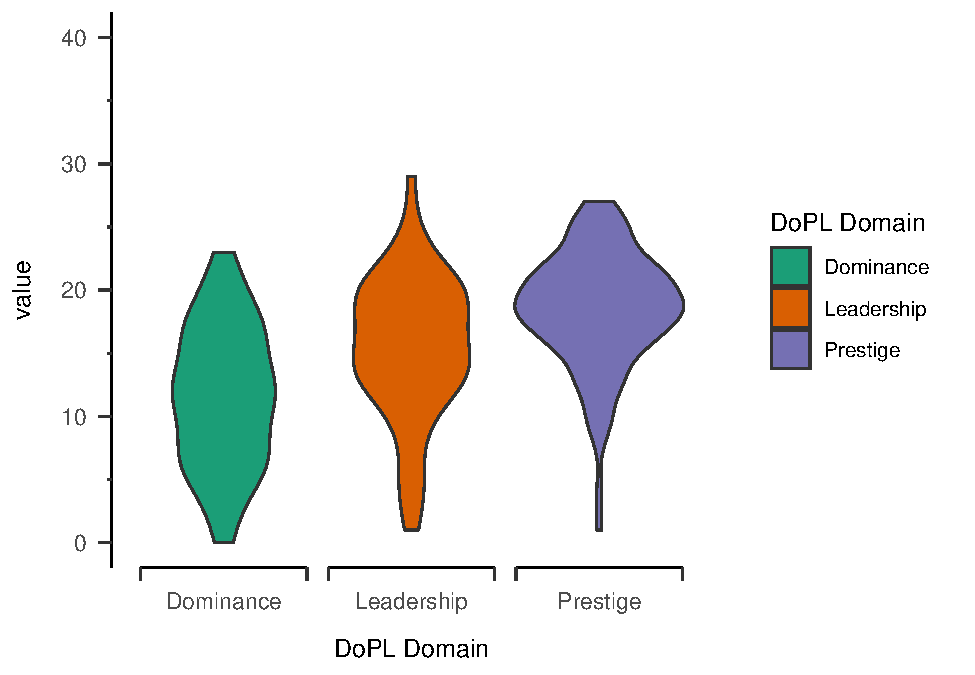
\includegraphics{DoPL-Experiment_files/figure-latex/unnamed-chunk-2-1.pdf}

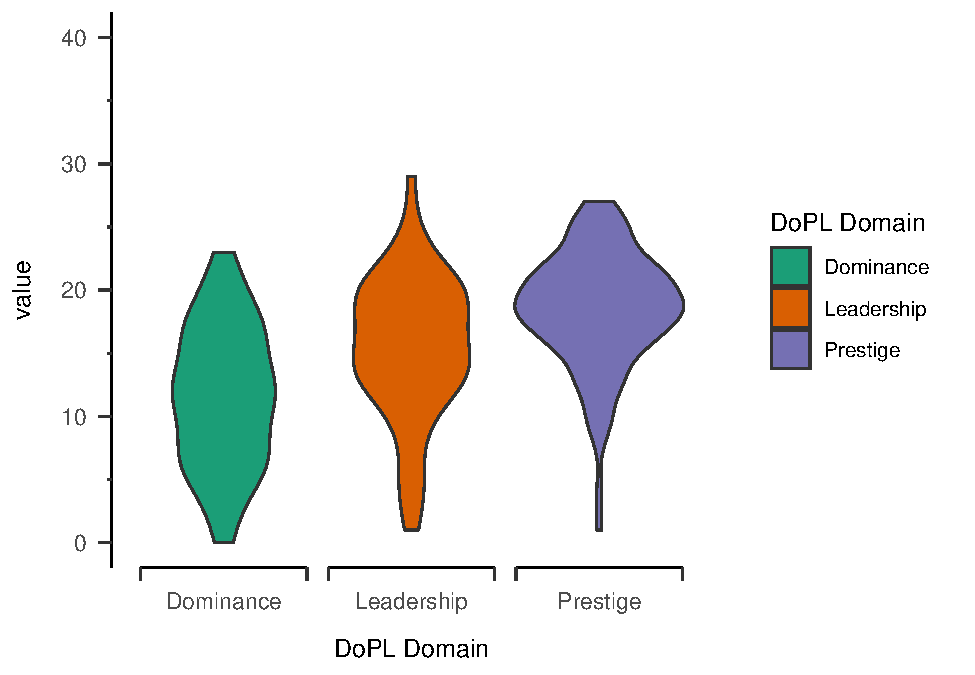
\includegraphics{DoPL-Experiment_files/figure-latex/unnamed-chunk-3-1.pdf} 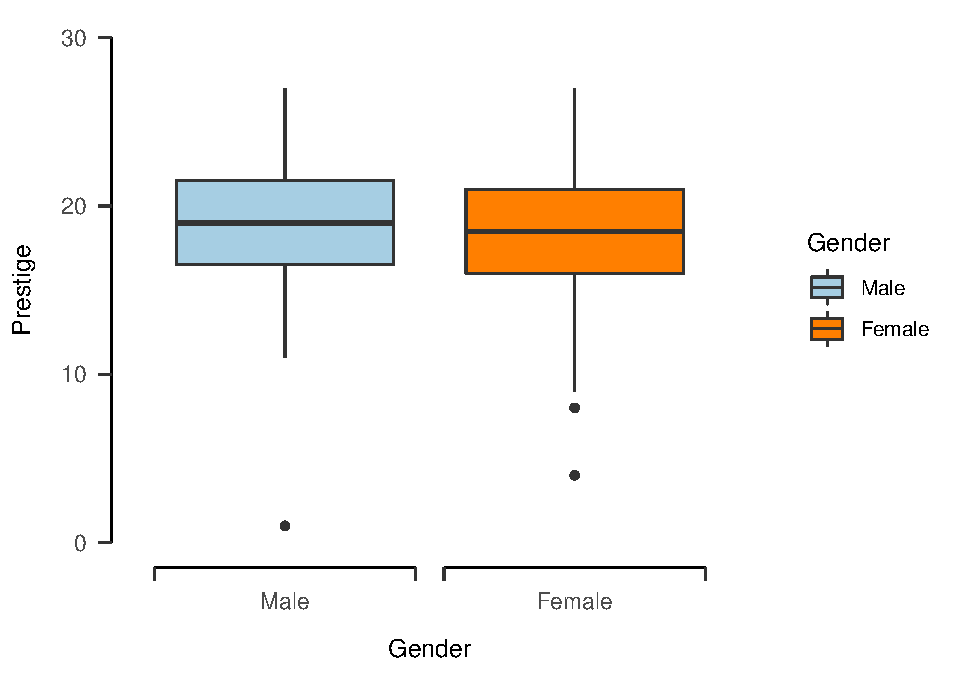
\includegraphics{DoPL-Experiment_files/figure-latex/unnamed-chunk-3-2.pdf} 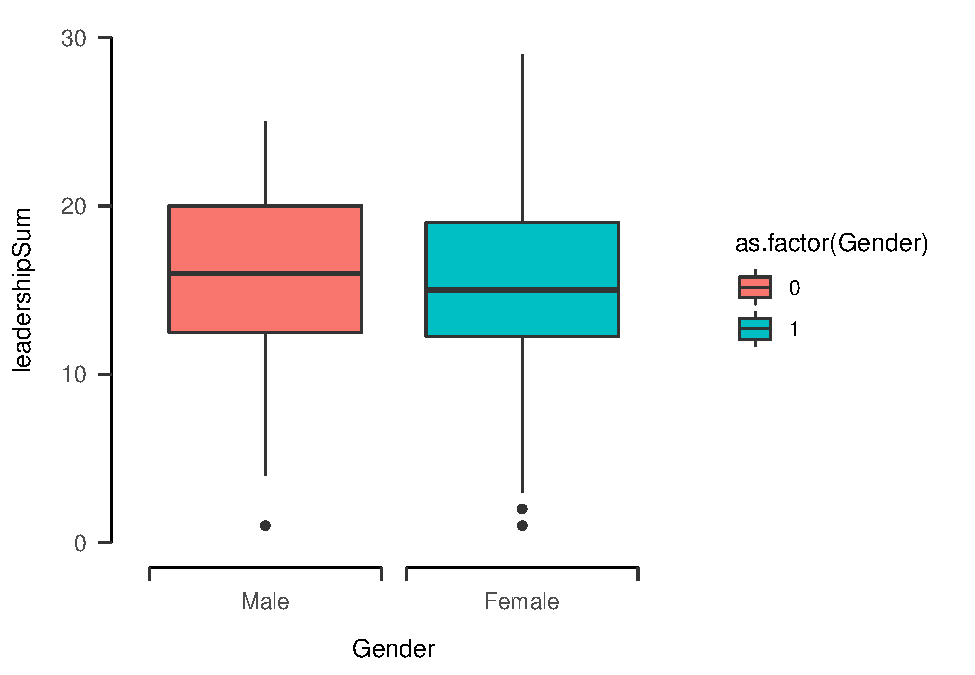
\includegraphics{DoPL-Experiment_files/figure-latex/unnamed-chunk-3-3.pdf}

\begin{table}[tbp]

\begin{center}
\begin{threeparttable}

\caption{\label{tab:unnamed-chunk-4}}

\begin{tabular}{llll}
\toprule
Parameter & \multicolumn{1}{c}{CI} & \multicolumn{1}{c}{CI\_low} & \multicolumn{1}{c}{CI\_high}\\
\midrule
b\_Intercept & 0.95 & 1.37 & 5.81\\
b\_dominanceSum & 0.95 & 1.07 & 4.91\\
b\_leadershipSum & 0.95 & -3.88 & -0.02\\
b\_Gender1 & 0.95 & -4.95 & -1.09\\
b\_Age & 0.95 & -4.80 & -0.96\\
\bottomrule
\end{tabular}

\end{threeparttable}
\end{center}

\end{table}

\begin{table}[tbp]

\begin{center}
\begin{threeparttable}

\caption{\label{tab:unnamed-chunk-5}}

\begin{tabular}{lllll}
\toprule
 & \multicolumn{1}{c}{Estimate} & \multicolumn{1}{c}{Est.Error} & \multicolumn{1}{c}{Q2.5} & \multicolumn{1}{c}{Q97.5}\\
\midrule
Intercept & 3.62 & 1.13 & 1.41 & 5.86\\
dominanceSum & 3.00 & 0.99 & 1.08 & 4.93\\
prestigeSum & 0.09 & 0.99 & -1.84 & 2.02\\
leadershipSum & -1.91 & 0.98 & -3.85 & 0.02\\
Gender1 & -3.02 & 0.99 & -4.95 & -1.08\\
Age & -2.86 & 0.99 & -4.78 & -0.93\\
\bottomrule
\end{tabular}

\end{threeparttable}
\end{center}

\end{table}

\begin{table}[tbp]

\begin{center}
\begin{threeparttable}

\caption{\label{tab:unnamed-chunk-6}}

\begin{tabular}{llll}
\toprule
Parameter & \multicolumn{1}{c}{CI} & \multicolumn{1}{c}{CI\_low} & \multicolumn{1}{c}{CI\_high}\\
\midrule
b\_ethicalPreference\_Intercept & 0.95 & 2.85 & 4.42\\
b\_ethicalPreference\_dominanceSum & 0.95 & 0.61 & 1.71\\
b\_financialPreference\_Intercept & 0.95 & 7.50 & 9.67\\
b\_financialPreference\_dominanceSum & 0.95 & 0.14 & 1.59\\
b\_socialPreference\_Intercept & 0.95 & 8.34 & 11.67\\
b\_socialPreference\_dominanceSum & 0.95 & 0.60 & 2.87\\
b\_healthAndSafetyPreference\_Intercept & 0.95 & 4.65 & 6.59\\
b\_healthAndSafetyPreference\_dominanceSum & 0.95 & 0.41 & 1.77\\
b\_recreationalPreference\_Intercept & 0.95 & 0.95 & 2.48\\
b\_recreationalPreference\_dominanceSum & 0.95 & 0.66 & 1.74\\
b\_recreationalPreference\_Gender1 & 0.95 & -1.83 & -0.47\\
b\_recreationalPreference\_Age & 0.95 & 0.06 & 0.87\\
\bottomrule
\end{tabular}

\end{threeparttable}
\end{center}

\end{table}


\end{document}
